\documentclass{report}
\usepackage[margin=1in, paperwidth=8.5in, paperheight=11in]{geometry}
%Math packages%
\usepackage{amsmath}
\usepackage{amsthm}
%Spacing%
\usepackage{setspace}
%Package to adjust indentation%
\usepackage{changepage}
\onehalfspacing
%Lecture number%
\newcommand{\lectureNum}{22}
%Variables - Date and Course%
\newcommand{\curDate}{March 28, 2017}
\newcommand{\course}{CS 240}
%Defining the example tag%
%\theoremstyle{definition}%
\newtheorem{ex}{Example}[section]
%Setting counter given the lecture number%
\setcounter{chapter}{\lectureNum{}}
%Package to insert code%
\usepackage{listings}
\usepackage{courier}
\usepackage{xcolor}
\lstset { 
    tabsize=2,
    breaklines=true,
    language=C++,
    backgroundcolor=\color{blue!8}, % set backgroundcolor
    basicstyle=\footnotesize\ttfamily,% basic font setting
}
%Package to draw trees%
\usepackage{tikz}


\begin{document}
%Note title%
\begin{center}
\begin{Large}
\textsc{\course{} | Lecture \lectureNum{}}
\end{Large}
\end{center} 
\noindent \textit{Bartosz Antczak} \hfill
\textit{Instructor: Eric Schost} \hfill
\textit{\curDate{}}
\rule{\textwidth}{0.4pt}
% Actual Notes%
\section{Finishing up Compression}
\subsection{Burrows-Wheeler Transform}
Achieves the best compression of any algorithm we have seen (at least on English text). BWT proceeds in three steps:
\begin{itemize}
\item Place all cyclic shifts of some text $S$ in a list $L$
\item Sort the strings in $L$ lexicographically
\item $C$ is the list of trailing characters of each string in $L$
\end{itemize}
\subsubsection{What will this do?}
The idea is, given $C$, we can generate the \textit{first column} of the array by sorting (i.e., the original encoded string). The decoding algorithm:
\begin{itemize}
\item Make an array of $A$ of tuples $(C[i], i)$
\item Sort $A$ by the characters, record integer in array $N$
\item Set $j$ to index of $\$$ in $C$ and $S$ to empty string
\item Set $j = N[j]$ and append $C[j]$ to $S$
\item Repeat Step 4 until $C[j] = \$$
\end{itemize}
\section{External Memory}
The final topic in CS 240 yo. Recall the memory hierarchy:
\begin{itemize}
\item Registers (very fast, very small)
\item cache L1, L2
\item Main memory
\item External memory
\end{itemize}
Our general idea will involve adapting our algorithms to take the memory hierarchy into account, avoiding transfers as much as possible.\\
We store data in a \textit{dictionary}, usually stored in a BST. A more efficient implementation of trees is a \textit{2-3 Tree}
\subsection{2-3 Trees}
A 2-3 Tree is like a BST with additional structural properties:
\begin{itemize}
\item Every internal node either contains one KVP (Key-Value Pair) and two children, or two KVPs and three children (with two KVPs $a$ and $b$, the children are structured as: $< a$, $a < \& < b$, $> b$)
\item The leaves are NIL (do not store keys)
\item All the leaves are at the same level
\end{itemize}
Searching through a 1-node is just like a BST. For a 2-node, we must examine both keys and follow the appropriate path.
\subsubsection{Insertion in a 2-3 tree}
First, we find the lowest internal node where the new key belongs. If the node has only 1 KVP, just add the new one to make a 2-node. Otherwise, order the three keys as $a < b < c$. Split the node into two 1-nodes, containing $a$ and $c$, and (recursively) insert $b$ into the parent along with the new link.
\begin{figure}[ht]
\begin{center}
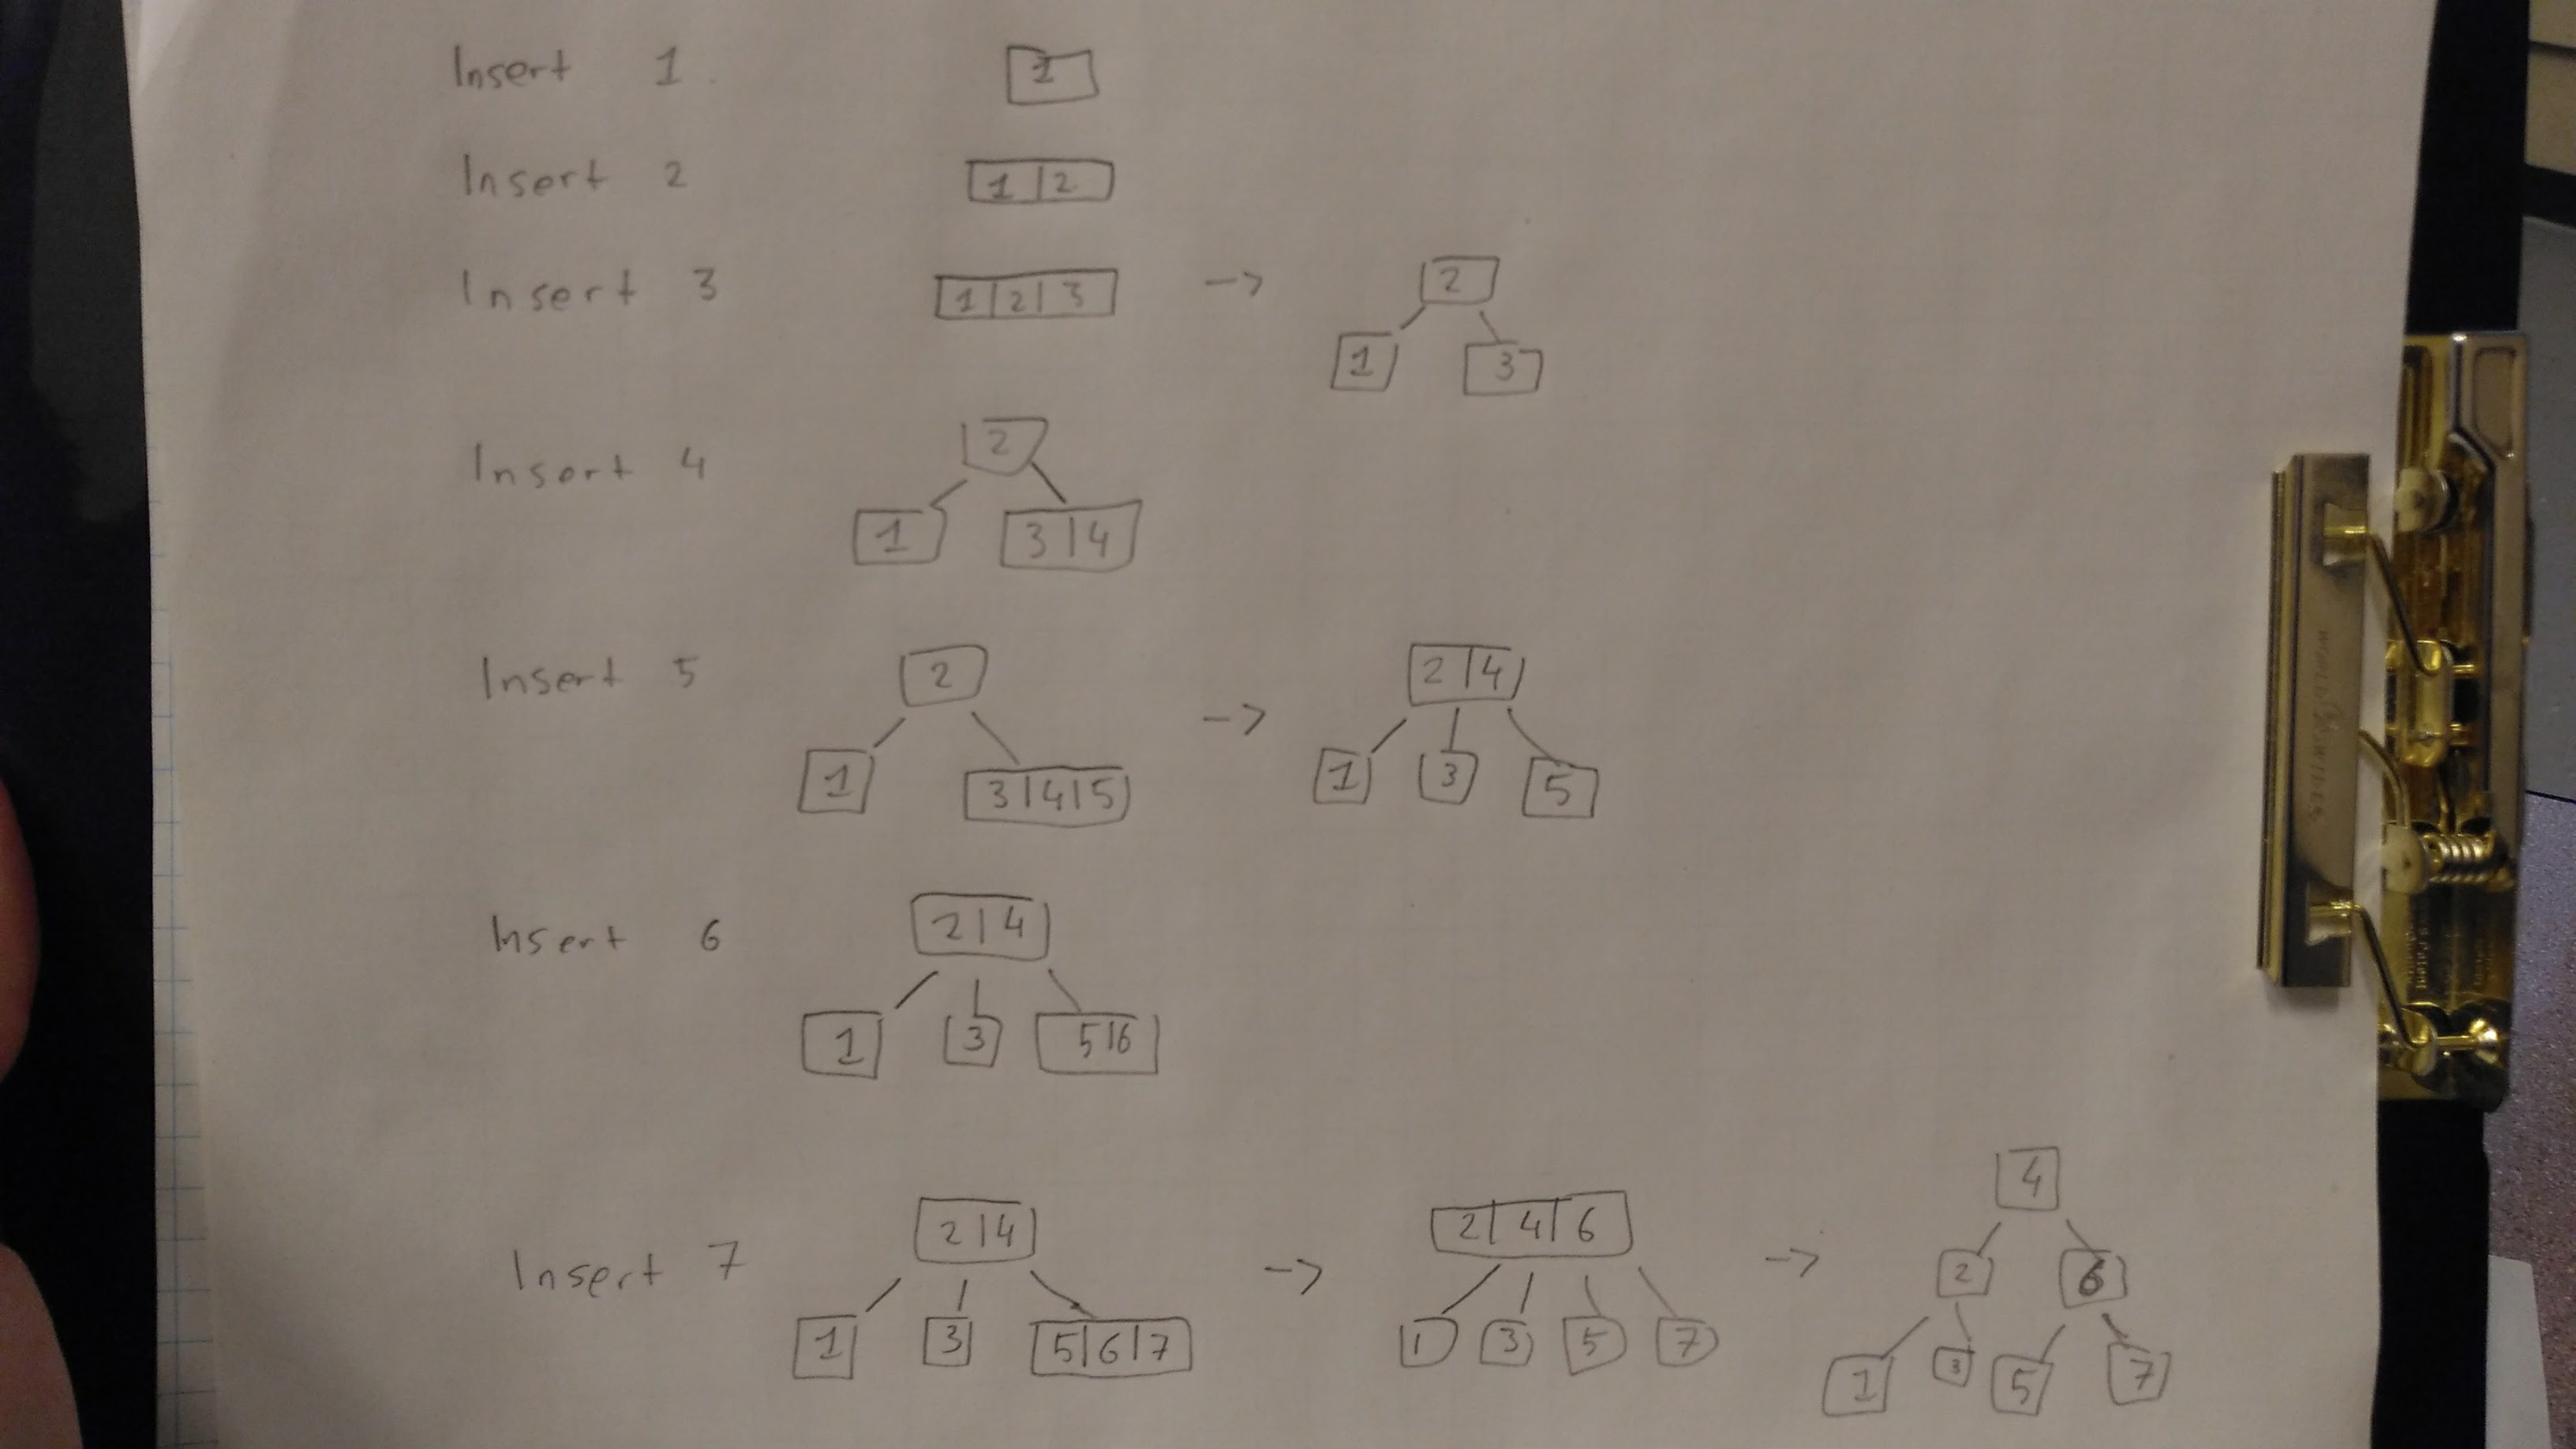
\includegraphics[scale=0.1]{img.jpg}
\end{center}
\end{figure}
\subsection{Deletion in a 2-3 tree}
Please refer to the course slides for how the process occurs.
\subsection{B-trees}
A 2-3 Tree is a specific type of an $(a,b)-$tree. An \textbf{(a,b)-tree of order M} is a search tree satisfying:
\begin{itemize}
\item Each internal node has at least $a$ children, unless it is the root. The root has at least 2 children
\item Each internal node has at most $b$ children
\item If a node has $k$ children, then it stores $k-1$ key-value pairs
\item Leaves store no keys and are at the same level
\end{itemize}
%END%
\end{document}